\chapter*{\centering LAMPIRAN}
\addcontentsline{toc}{chapter}{LAMPIRAN}

\section*{Lampiran 1: Contoh Lampiran Kode}
\addcontentsline{toc}{section}{Lampiran 1: Contoh Lampiran Kode}
\lstinputlisting[language=Python]{Kode/pdospy.py}
\pagebreak

\section*{Lampiran 2: Contoh Cara Menyusun Banyak Gambar}
\addcontentsline{toc}{section}{Lampiran 2: Contoh Cara Menyusun Banyak Gambar}

\begin{figure}[h]\hspace{-2em}
    \centering
    \begin{subfigure}{.3\linewidth}
      \centering
      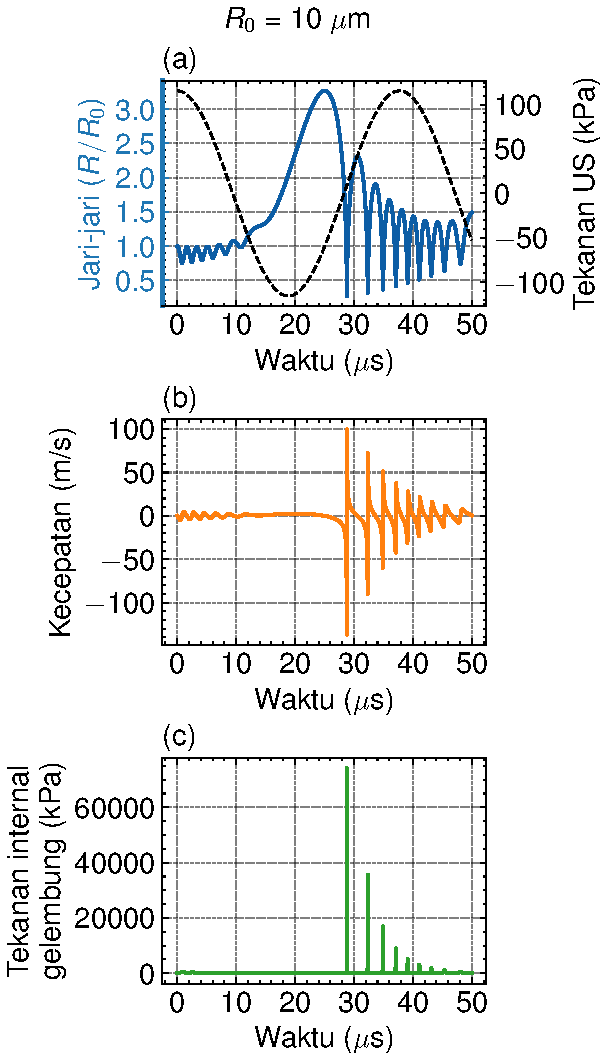
\includegraphics[width = 5.5cm]{Gambar/10.pdf}
    \end{subfigure}
    \hspace{1.5em}
    \begin{subfigure}{.3\linewidth}
      \centering
      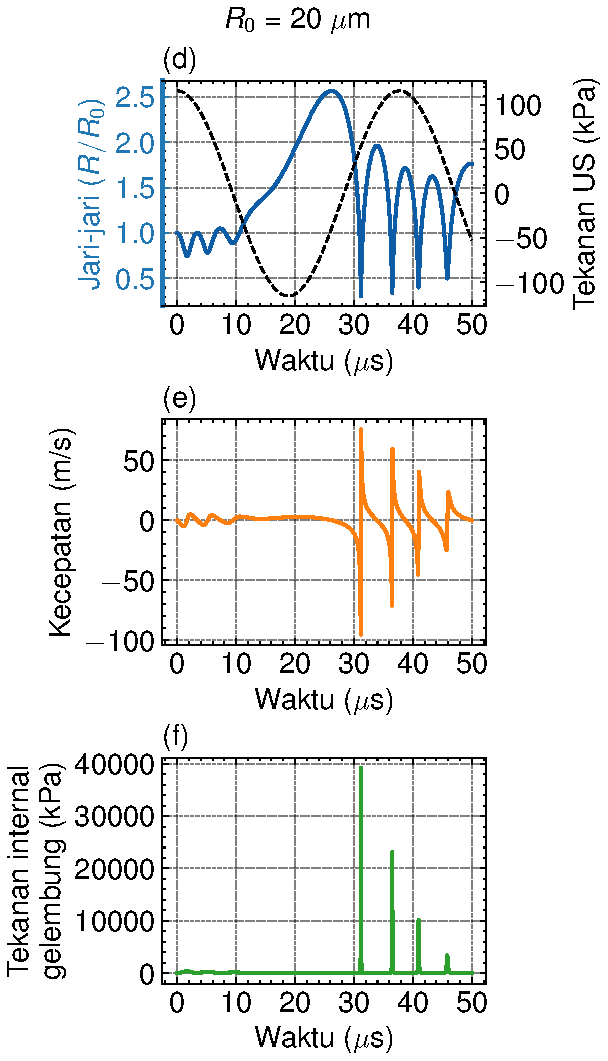
\includegraphics[width = 5.5cm]{Gambar/20.pdf}
    \end{subfigure}
    \hspace{1.5em}
    \begin{subfigure}{.3\linewidth}
      \centering
      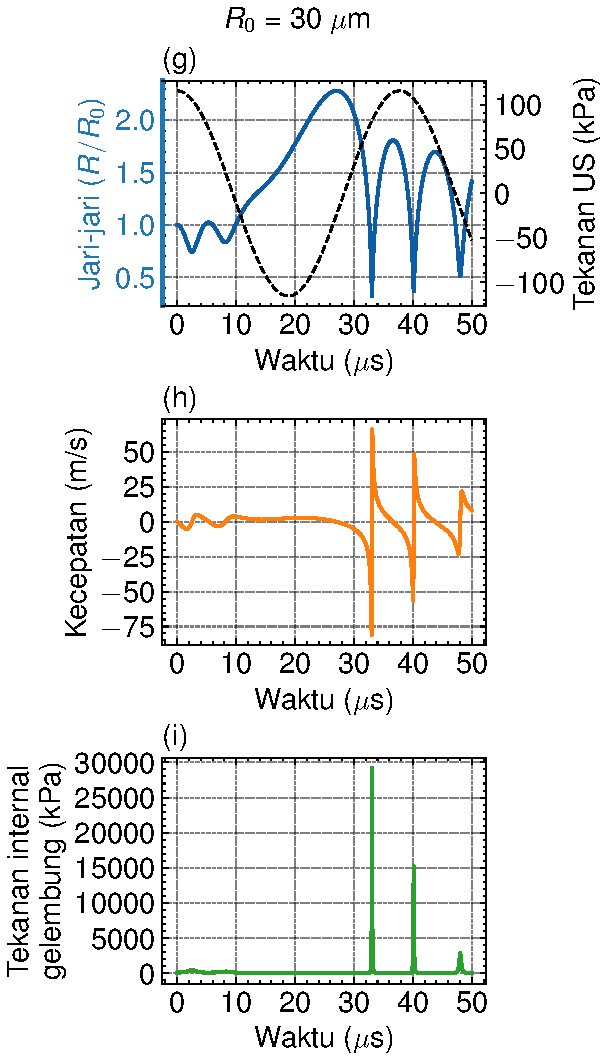
\includegraphics[width = 5.5cm]{Gambar/30.pdf}
    \end{subfigure}
  \end{figure}

\section*{Lampiran 3: Contoh Cara Menyisipkan Gambar pada Gambar}
\addcontentsline{toc}{section}{Lampiran 3: Contoh Cara Menyisipkan Gambar pada Gambar}
  \begin{figure}[H]
    \centering   
    \begin{overpic}[width=14cm]{Gambar/PDOSid.pdf}
       \put(76,14){
\includegraphics[width=1.25cm]{Gambar/gband.png}}  
    \end{overpic}
  \end{figure}
\pagebreak

\section*{Lampiran 4: Contoh Diagram}
\addcontentsline{toc}{section}{Lampiran 4: Contoh Diagram}
\begin{figure}[H]
  \centering
  \begin{tikzpicture}[node distance=2cm]
  \node (ini) [process, yshift=0.4cm] {Inisiasi};
  \node (relax) [process, below of=ini, yshift=0.4cm] {Relaksasi Struktur};
  \node (eq) [process, below of=relax, yshift=0.4cm] {Ekuilibrium};
  \node (s) [decision, below of=relax, yshift=-1.4cm] {Stabil?};
  \node (res) [process2, left of=s, xshift=-2cm] {\textit{Velocity scaling}};
  \node (prod) [process, below of=s, yshift=-0.2cm] {Produksi};
  \node (post) [process, below of=prod, yshift=0.4cm] {Hasil};
  
  \draw [arrow] (ini) -- (relax);
  \draw [arrow] (relax) -- (eq);
  \draw [arrow] (eq) -- (s);
  \draw [arrow] (s) -- node[anchor=south] {Tidak} (res);
  \draw [arrow] (res) -- +(-2,0) |- (eq);
  \draw [arrow] (s) -- node[right] {Ya} (prod);
  \draw [arrow] (prod) -- (post);
  \end{tikzpicture}
  \end{figure}
  